\chapter{Methodology}

\Olga{Start each chapter with a para describing what it's about.} This chapter describes the methodology we followed to ... Section~\ref{sec:data_collection} describes two key data sources such as Stack Overflow and GitHub and offers the details on the data collection process. Section~\ref{sec:data_storage} ... Section~\ref{sec:data_aggregation} ... Section~\ref{sec:data_cleaning} ...  Section~\ref{sec:topic_modeling} ... Section~\ref{sec:expertise_survey} ...
Section~\ref{sec:algo_design} ...
And finally, Section~\ref{sec:tools} ...

\section{Data Collection} \label{sec:data_collection}

    When mining GitHub \Olga{add a reference to GitHub website} and Stack Overflow \Olga{add a reference to Stack Overflow website}, a natural starting point is to use GHTorrent \cite{gousios2013ghtorent} and SOTorrent \cite{baltes2018sotorrent} as data sources.
    
    \subsection{Stack Overflow Data}
    
        SOTorrent\footnote{\label{SOTorrent}\url{https://empirical-software.engineering/projects/sotorrent/}} is an open data set based on periodic, official Stack Overflow data dumps. SOTorrent was built for the purposes of mining and analyzing the evolution of Stack Overflow posts. A new version of this data set based on the latest Stack Overflow data dump is released every 3 months. Each version of the SOTorrent data set can be downloaded from Zenodo\footnote{\label{SOTorrent_Zenodo} \url{https://zenodo.org/record/2273117}}. The latest versions of the SOTorrent data set are also available online, and can be queried through Google BigQuery\footnote{\label{BigQuery} \url{https://bigquery.cloud.google.com/dataset/sotorrent-org:2018_12_09}}.
        
        When downloading the SOTorrent data set, the version from \textit{December 9th 2018} was used, as it was the latest version available at the start of the project. The SOTorrent data set has its files organized into tables. Not all tables were downloaded, as certain tables related to post evolution (e.g., \texttt{PostHistory} and \texttt{PostVersion} tables) were unrelated to the expertise learning task. The tables downloaded included \Olga{use texttt for tables} \texttt{Users}, Posts, PostLinks, PostType, PostReferenceGH, Comments, CommentUrl, GHMatches, Tags, Badges and Votes, totaling 29 GB of compressed raw data. After downloading and uncompressing all relevant data files, the data set contained just shy of 100 GB of data.
        
    \subsection{GitHub Data}
    
        GHTorrent\footnote{\label{GHTOrrent}\url{http://ghtorrent.org/}} is also an open data set, which mirrors the data offered through the GitHub REST API\footnote{\url{https://developer.GitHub.com/}}. GHTorrent collects data from all public projects available on GitHub and releases a new version of MySQL data dumps every month, while it also offers daily data dumps through MongoDB. Each version of MySQL data can be downloaded from GHTorrent\footnote{\label{GH_dowload}\url{http://ghtorrent.org/downloads.html}}. GHTorrent data can also be queried online, as it is available via a DBLite web interface\footnote{\label{GH_query}\url{http://ghtorrent.org/dblite/}}. 
            
        When downloading the GHTorrent data set, we used the version from \textit{March 1st 2019}, as it was the latest version available at the time of download. The data set has its files organized into large tables stored in compressed CSV files, totaling 96,557 \Olga{use comma as a thousands separator} MB of compressed data. All files were downloaded and uncompressed which resulted in 21 raw data tables totaling over 400 GB of data.

\section{Data Storage} \label{sec:data_storage}

    \subsection{Database Setup and Data Import}
        
        A MySQL database was the obvious choice of database, as both data sources come with SQL scripts performing table creations, data imports and general database manipulations\footnote{\label{SO_sql} \url{https://GitHub.com/sotorrent/db-scripts/tree/master/sotorrent}} \footnote{\label{GH_sql} \url{https://GitHub.com/gousiosg/GitHub-mirror/tree/master/sql}}. Managing disk space during the data import phase represented a challenge, as the raw, uncompressed data files totaled up to over 500 GB. Importing of the data into the database was not achieved all at once, but rather through several iterations of uncompressing only a few data files. After a file was uncompressed and the table was successfully imported into the database, we deleted its raw CSV or XML file to free up disk space. 
        
        During the data import phase, we discovered that using \textit{MyISAM} over \textit{InnoDB} as the database engine is more favorable, since there was a significant execution time difference between the two database engines when importing large amounts of data into the MySQL database. \textit{MyISAM} database engine does not support foreign keys constraints, while it supports table-level locking. On the other hand \textit{InnoDB} supports foreign key constraints and row-level locking. \textit{MyISAM} is preferred when performing tasks that require fast import and querying speed, while \textit{InnoDB} being the default database engine for MySQL is more optimal for regular operations. For this particular reason, we imported all of the large raw data files into the database using the \textit{MyISAM} database engine. After all necessary database manipulations have been performed, the database engine was changed back to the default engine, \textit{InnoDB}, to allow foreign key constraints to be enforced. 
     
        \todo{Add table contains descriptions for each sql table's content}
      
        \begin{figure}[!ht]
          \centering
          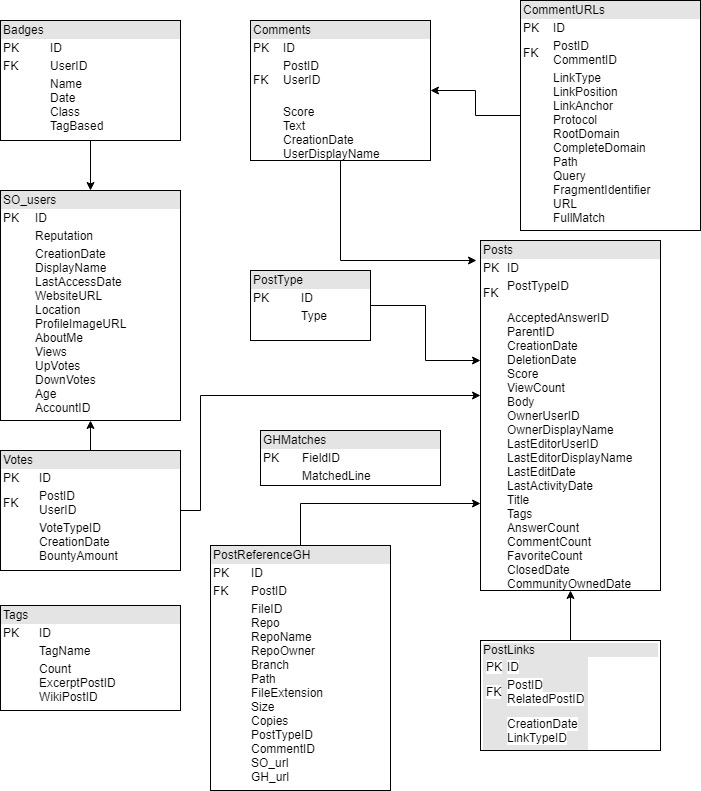
\includegraphics[width=0.9\textwidth]{SO_DB_schema.jpg}\\
          \caption{Database schema for Stack Overflow data.}
          \label{fig:so_schema}
        \end{figure}
        
 
        \begin{figure}[!ht]
          \centering
          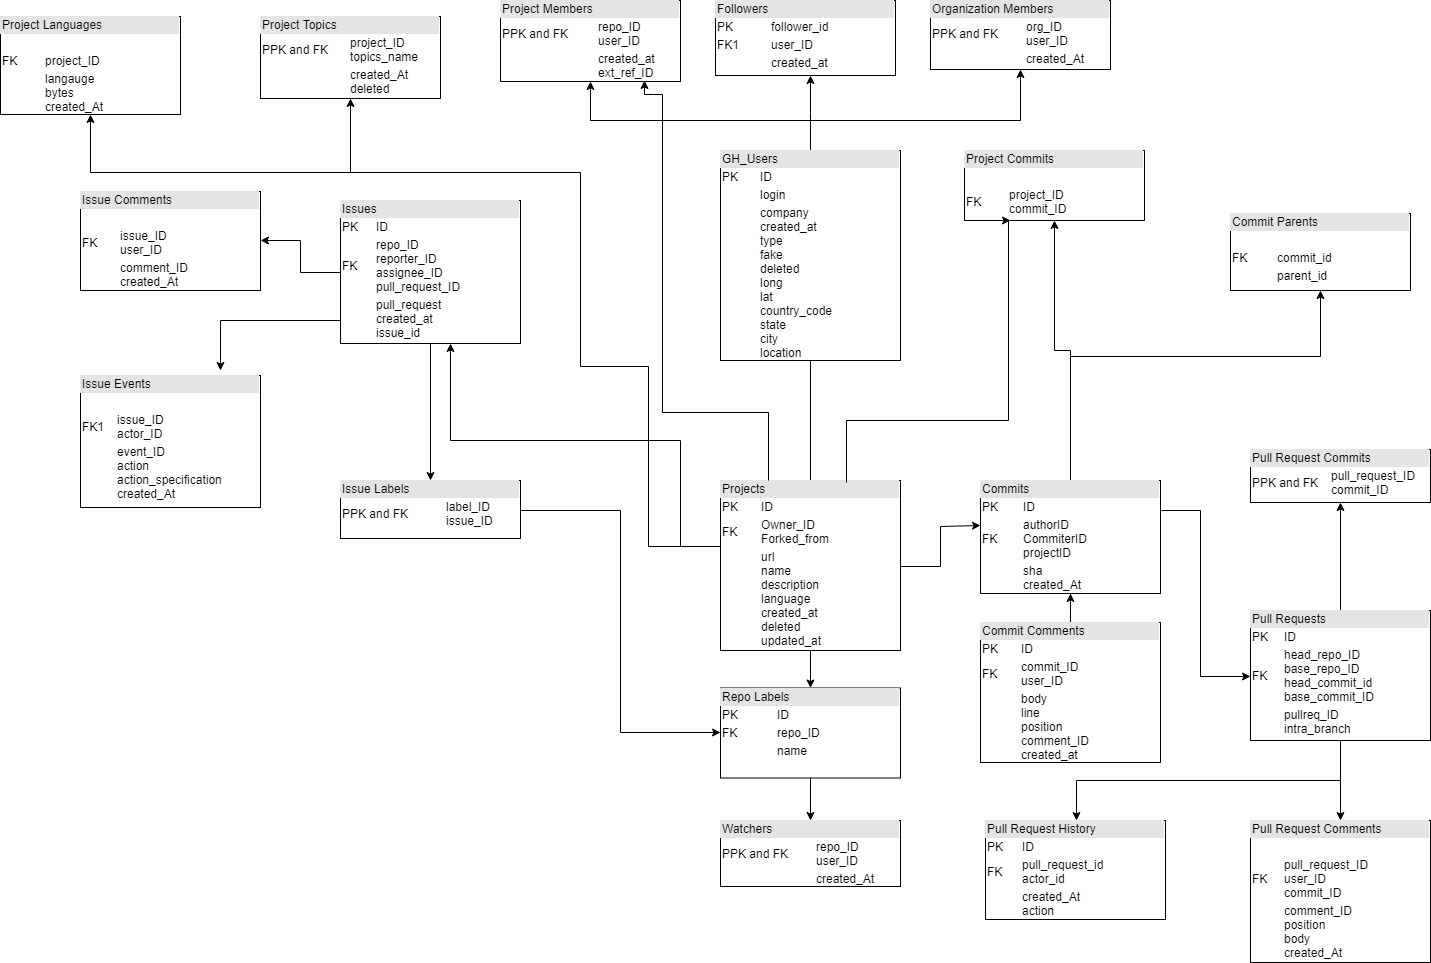
\includegraphics[width=\textwidth]{GH_DB_schema.jpg}\\
          \caption{Database schema for GitHub data.}
          \label{fig:gh_schema}
        \end{figure}
        
        \todo{Re-do GitHub DB schema}
        
        Figure \ref{fig:so_schema} and \ref{fig:gh_schema} show the database schema and all attributes within each table of the SOTorrent and respectively the GHTorrent data set. All tables from GHTorrent are shown in figure \ref{fig:gh_schema}, while only the relevant tables from SOTorrent are shown in figure \ref{fig:so_schema}. 


    \subsection{Linking together GHTorrent and SOTorrent}\label{Linking_SO_GH}
    
        In order to perform cross-platform analysis of GitHub and StackOverflow,  we need to link  GHTorrent and SOTorrent datasets. \Olga{Choose one ``dataset'' or ``data set'' and use consistently throughout the thesis}. This task requires identifying the same user's accounts on both platforms. Looking at relevant literature on this problem, we can identify the task of \textit{identity merging}, which consists of identifying the same person in two or more different environments. Vasilescu et al. \cite{vasilescu2013stackoverflow} researched this problem rigorously and after careful consideration of limiting the number of false positives they used email addresses to determine user identity. In 2013, at the time of publishing their work, email addresses were present in the GitHub dataset, while in the Stack Overflow dataset email addresses were not publicly released, but their MD5 hashes were available. Vasilescu et al. \cite{vasilescu2013stackoverflow} decided to ``merge (i.e., link) a GitHub and a Stack Overflow user if the computed MD5 hash [of the email in GitHub] is identical to the MD5 email hash [of Stack Overflow users]''. This resulted in 93,771 GitHub users being linked to Stack Overflow \Olga{Use Stack Overflow (not StackOverflow)}. Vasilescu et al. \cite{vasilescu2013stackoverflow} further investigated and came to the conclusion that out of 93,771 linked users only 46,967 users were active at the time. The linked dataset alongside a replication package has been made publicly available by the authors\footnote{\label{bodgan_dataset}\url{https://www.win.tue.nl/mdse/stackoverflow/}}. This dataset has been used multiples times to analyze the interaction of GitHub and Stack Overflow data \cite{badashian2014involvement} and \cite{lee2017github}, thus it became the backbone of the data sampling process behind linking together GitHub and Stack Overflow users.  

        There was one major problem with using Vasilescu et al. \cite{vasilescu2013stackoverflow}'s dataset. The replication package contained a dataset linking GitHub email addresses to Stack Overflow user IDs, without fully mapping GitHub user IDs to Stack Overflow user IDs, therefore, we needed to map GitHub email addresses to user IDs. This mapping was possible when Vasilescu et al. \cite{vasilescu2013stackoverflow} published their work, but after March 2016 GHTorrent was not allowed to store email addresses in their open datasets, as it violated the EU General Data Protection Regulation (GDPR). Our solution to this problem was to download the \texttt{User} table data from GHTorrent's last available version that still contains email addresses of GitHub users in the data set. This older version of GHTorrent is dated \textit{February 1st 2016}, and it was downloaded, then imported into the MySQL database. We prefromed a manual check on matching user IDs and login names between the \texttt{User} table's March 2019 and February 2016 versions. This manual check made sure that the user IDs from both versions of the table are referring to the same login name. If this was not the case, the user was dropped from the dataset, due to inconsistency of the two versions of table. This manual check assured consistency in the data linkage between Stack Overflow and GitHub users, but resulted in the removal of over 10,000 users from the original 93,771 users linked. The final dataset contains 83,550 user accounts being linked between the two platforms, offering a unique GitHub user ID to Stack Overflow user ID mapping. It can be speculated that removed users either deleted or changed the login name of their GitHub account between 2016 and 2019, thus causing the inconsistency in the two versions of the \texttt{User} table.
        
    \subsection{Discarding Unlinked Data}
    
       As mentioned in Section~\ref{sec:data_collection}, the total size of the GHTorrent dataset was over 400 GB of data, while SOTorrent contained close to 100 GB of data. In order to make data querying and processing more efficient, we needed to perform a data reduction on the full dataset. 
       %In order to perform analysis on the linked data between GitHub and Stack Overflow, only successfully linked data is needed. 
       We filtered out unlinked data by iterating through each existing table in the database and keeping only the observations that are connected or related to users with a user ID present in the list of 83,550 unique user IDs linked. Discarding unlinked data reduced the size of the data set and allowed only linked data to be analyzed. This process reduced the size of the MySQL database from over 500 GB of data to 122 GB.
        
\section{Data Aggregation} \label{sec:data_aggregation}

    The end goal of the analysis on Stack Overflow and GitHub data was to create topic models capable of deciphering the hidden patterns of underlying topics that represent a user's expertise and activity on a platform. Tian et al.~\cite{tian2013predicting} modeled user topical interest and expertise by building LDA models on user activity (user profile) data. They have showed that a Stack Overflow user's expertise can be extracted using a topic model applied over a set of textual documents consisting of the user's activity on the platform collected into a user profile.

    In order to perform cross-platform analysis of GitHub and Stack Overflow users' expertise, we modeled their expertise through LDA models. LDA topic models are fitted on a set of documents. In order to fit topic models on GitHub and Stack Overflow user data, one needs to define what a document consists of, and how to extract a user's profile from a platform such as GitHub or Stack Overflow. This process is explained in the following three subsections (i.e., Section~\ref{SO_userProfileExtraction}, Section~\ref{GH_userProfileExtraction}, and Section~\ref{past_recent_full_segm}).
    
    \subsection{Extracting Stack Overflow User Profiles} \label{SO_userProfileExtraction}
    
        When deciding on how to create documents for the LDA topic model, we define a document as a single user profile. Each user who is present in the dataset of 83,550 linked users described in Section~\ref{Linking_SO_GH} has one document (user profile) describing their activity on Stack Overflow. This document contains all of their activity on the platform. Extracting a user's activity (user profile) from all the public data stored about a user started by inspecting each table of the SOTorrent database schema \ref{fig:so_schema} for attributes that contain relevant and meaningful textual information about a user. The relevant textual attributes included into the user profiles are \textit{badge names} obtained by a user, the \textit{about me} description from the user profile, \textit{questions} posted by a user, \textit{answers} given by a user, \textit{titles} and \textit{tags} of posts that a user participated in, and \textit{comments} made by a user to any post. 
          
        \begin{table}[!htbp]
            \centering
            \label{tab:SO_userProfileExtraction}
            \caption{Stack Overflow user profile extraction.}
            \vspace{6pt} % Required to get proper spacing between caption and table
            \begin{tabular}{|p{3.3cm}|p{2.7cm}|p{8cm}|}
               \toprule
               \textbf{Attribute Name} & \textbf{Attribute(s)} & \textbf{Derivation} \\
               \toprule
                Badges & Badges.Name & Concatenation of list of badges obtained by the user \\
                About Me & Users.AboutMe & Stack Overflow user profile's about me description \\
                Post Answer & Posts.Body, AcceptedAnswerId & Take a user's each answer and concatenate it with the question that it is related to  \\
                Post Question & Posts.Body & Take a user's each question and concatenate it with the accepted answer it is related to  \\
                Title and Tags for Questions & Posts.Tags, Posts.Title & Concatenate the post tags and title for each question that the user asked \\
                Title and Tags for Answers & Posts.Title, Posts.Tags & Concatenate the post tags and title for each answer that the user provided \\
                Comments & Comments.Text, Posts.Body, Posts.Title & Take a user's each comment and concatenate it to the post (question or answer) it is related to \\
               \bottomrule
            \end{tabular}
        \end{table} 
        
        A detailed description on how each attribute from the user profiles was processed can be found in Table~\ref{tab:SO_userProfileExtraction}. For the \textit{Post Answer} attribute in order to restore the semantic context of the user's answer, the question being asked is concatenated before the answer, thus creating a question-answer pair. For the same reason the \textit{Post Question} attribute is getting the accepted answer concatenated in, thus adding more contextual clarity to the user's question. This process is being applied to the \textit{Comments} attribute as well, creating question-comment or answer-comment pairs, depending on what the comment is related to. At the end of this process all attributes in the user profile are merged into one large document representing a user's full activity on the SO platform. 
        
    \subsection{Extracting GitHub User Profiles} \label{GH_userProfileExtraction}
    
        Each user who is present in the dataset of 83,550 linked users described in Section~\ref{Linking_SO_GH} has one document (user profile) describing their activity on GitHub. We extracted a user profile by inspecting each table of the GHTorrent database schema~\ref{fig:gh_schema} for attributes that contain relevant textual information about a user. The textual attributes selected to be part of the GH user profile data include the \textit{names}, \textit{labels}, \textit{languages} used,  \textit{description of the repository} that a user owns, as well as their \textit{commit} and \textit{pull request comments} posted on GitHub. 
        
        \begin{table}[!htbp]
            \centering
            \caption{GitHub user profile extraction.}
            \label{tab:GH_userProfileExtraction}
            \vspace{6pt} % Required to get proper spacing between caption and table
            \begin{tabular}{|p{3.3cm}|p{3.3cm}|p{7cm}|}
               \toprule
               \textbf{Attribute Name} & \textbf{Attribute(s)} & \textbf{Description} \\
               \toprule
                Project Name, Description and Metadata & Projects.[name, description, language], Repo-Labels.name & Description of each user's project together with the repository's name, description, languages used, repository labels it contains.\\  
                Commit-Comments & Commit-Comments.body & List of user's commit comments.\\
                Code-review Comments & Pull-Request-Comments.body & List of user's code review (pull request) comments. \\
               \bottomrule
            \end{tabular}
        \end{table}
        
        \Olga{I suggest to use Description instead of Derivation and provide descriptive statement of what that attribute is. I have tried this for Table 3, please do same for Table 2.}
        A detailed description on how each attribute from the user profiles was processed can be found in Table~\ref{tab:GH_userProfileExtraction}. Attributes such as the name, description and labels of a repository, alongside the programming languages used are valuable information describing the content of a repository on GitHub. Discussion between users in the form of comments to commits and pull request comments are also essential to establish contextual details about the project, thus these attributes have been included in the user profile. All the above listed attributes get merged into one large document representing a user's full activity on the platform. 
        
    \subsection{Creating Time Based User Profiles} \label{past_recent_full_segm}
        After defining how to extract user profiles from both Stack Overflow and GitHub, it is worth factoring in a \textit{timeline} into the user profile. The simplest approach would be to model recent and past activity of users by splitting their activity into before and after a specific date. Being able to model past and recent user profile data separately creates opportunities for comparison analyses to be done on the evolution of expertise of GitHub and Stack Overflow users. We decided to define recent activity as the activity performed by a user in the last 3 years. Since our study took place in 2019, we split user activity profile into recent and past, i.e., any activity dated before \textit{January 1st 2016} is considered as \textit{past activity}, while activity that took place after \textit{January 1st 2016} is defined as \textit{recent activity}. 
        %the split between past and recent activity was created by any user profile data being dated before or after \textit{January 1st 2016}.
        
        Based on our definition of recent activity, three types of datasets have been created: 1) data containing only recent activity, 2) only past activity data, and 3) both past and recent activity data. The past activity dataset includes data from the day the platform started recording data up to \textit{January 1st 2016}, while the recent dataset contains data only after \textit{January 1st 2016}, up to the date of data collection. The ``full'' dataset contains all the data for a platform, and has no time segmentation. In the following sections this data segmentation will be referred to as \emph{past, recent and full}, alongside the platform abbreviation SO and GH for Stack Overflow and GitHub, respectively, i.e.,  \emph{GH-past, GH-recent, GH-full, SO-past, SO-recent and SO-full}.

\section{Data Cleaning}\label{sec:data_cleaning}

    Textual data on Stack Overflow and GitHub contains a large variety of domain-specific (i.e., software engineering) terminology mixed with source code. Stack Overflow posts contain rich software artifacts such as code snippets, text blocks explaining problems and solutions using text and source code, comments which can be associated with a question or an answer, and hyperlinks to references such as API documentation or a publication explaining an answer.  Liao et al. \cite{liao2019status} in their study on GitHub mention that developers on GitHub ``talk about project bugs, enhancements, and tasks in issue discussions''. The authors stated that a text corpus built on GitHub data is most likely  to contain ``plenty of code, warnings, messages, and technical terminology in addition to more general natural language [...] which allow for easy detection of status and/or relevant expertise''.
    
    We can conclude that textual data on both GitHub and Stack Overflow captures a variety of aspects of software development, but its technical terminologies, mix of text and source code makes it difficult to extract the proper textual data to be analyzed. When performing text pre-processing on both sources of data, we need to find the right balance between more than a dozen pre-processing techniques in order to clean up the data just the right way, without removing software engineering domain-specific words and damaging the contextual details of software artifacts. Deciding on a precise set of techniques for the pre-processing routine can be a challenging task, thus we conducted an extensive research on what text pre-processing techniques have been previously used for analyzing GitHub and Stack Overflow data.
    
    Tian et al. \cite{tian2013predicting} pre-processed textual data by performing tokenization, stop-word removal and stemming. They also split function names from cleaned up source code related keywords in the text processing phase.
    
    Campbell et al. have also addressed the challenge of data pre-processing. In their
    book chapter~\cite{campbell2015latent} on extracting topics from software engineering data, they say that generally those who use LDA apply the following pre-processing steps: ``loading text, mapping text into final textual representation, [perform] lexical analysis of the text, optionally removing stop words, optionally stemming, building a vocabulary, optionally removing uncommon or very common words and mapping each text document into a word-bag''. \todo{re-write big quote}\Olga{I think the quote is fine.}
    
    Treude and Wagner \cite{treude2019predicting} have performed similar but separate pre-processing routines on Stack Overflow and GitHub data. Their Stack Overflow data cleaning routine consists of removing line breaks, code blocks, all HTML tags, replacing HTML symbols and strings indicating special characters with their corresponding character, and replacing sequences of whitespace with a single space. Their GitHub pre-processing routine is the same as the Stack Overflow data cleaning routine, with a few extra steps, such as removing vertical and horizontal lines, code comments, characters denoting sections headers, characters that indicate formatting or links. 
    
    Efstathiou et al. \cite{efstathiou2018word} converted text from Stack Overflow into lowercase, removed code snippets and HTML tags, then performed a ``conservative punctuation removal, keeping symbols that often appear in programming commands, such as ``+'' and ``\#'' which are essential for differentiating ``C'', ``C++'', and ``C\#'' from one another''. 
    
    Boyd-Graber et al.'s book chapter~\cite{boyd2014care} recommends HTML symbol and stopword removal, then normalizing strings by converting to lower case and applying any kind of stemming algorithm, then applying tokenization and any kind of phrase detection algorithm as the proper pre-processing routine before fitting topic models on textual data.
    
    Liao et al. \cite{liao2019status} analyzed issue discussions on GitHub, and in their pre-processing steps they filtered out code-specific language, which was enclosed in HTML tags. The authors then removed short posts contained less than five tokens and distinguished between data generated by developers who never committed code to a project, and those who did. 
    
    Based on the existing state-of-the-art data cleaning routines used when working with software engineering domain-specific textual data, we developed a \emph{user-level} and a \emph{corpus-level} pre-processing routines. 
    
    \subsection{User-Level Text Processing}
    
        The user-level pre-processing routine is executed on each user's aggregated textual data during the user profile extraction processing described in Section~\ref{SO_userProfileExtraction} and Section~\ref{GH_userProfileExtraction}. The user-level routine involved the removal of HTML links, symbols and tags, proceeded by stop-word, mentions (using @) and multiple white space removal. Finally, a tokenization technique is applied, then individual tokens consisting of only numbers or punctuation with no words present in the token are removed. This data processing routine is executed on the already aggregated (concatenated) data obtained using the description in Section~\ref{SO_userProfileExtraction} and Section~\ref{GH_userProfileExtraction}.
        
    \subsection{Corpus-Level Text Processing}
    
        The corpus-level pre-processing routine is executed on each individual text corpus (GH-past, GH-recent, GH-full, SO-past, SO-recent and SO-full, as described in Section~\ref{past_recent_full_segm}) before the model fitting, but after the data aggregation process. The corpus-level pre-processing includes tokenization, standardization of tokens, frequent phrase detection, then removing tokens that include only numbers and punctuation (if any). A subset of symbols and punctuation are also removed, keeping symbols such as ``+'', ``\_'', ``.'' and ``\#'', which often appear in programming contexts. Finally, rare and very common tokens are removed by filtering out tokens that occur in less than 10 documents or more than 50\% of the documents. In this context, standardization of tokens means re-writing common tokens spelled multiple ways as a unique token. Examples of such common tokens include ``node.js'', ``node-js'', ``node\_js'' for ``nodejs''; ``angular.js'', ``angular-js'', ``angular\_js'' for ``angularjs''; or ``js'' for ``javascript', and many more. A list of the most frequent phrases detected in the GH-full and SO-full datasets can be found in Appendix~\ref{frequentExpressions}. These common phrases used in the software engineering domain have a different meaning as a phrase (bigram), thus they have been re-written as a single word (unigram), using a ``\_'' character connecting the phrases. As a final note on data cleaning, both user- and corpus-level pre-processing routines are designed based on common best practises of previous data cleaning routines (e.g., \cite{tian2013predicting}, \cite{campbell2015latent}, \cite{treude2019predicting}, \cite{efstathiou2018word}, \cite{boyd2014care}, and \cite{liao2019status}).

\section{Topic Modeling\label{sec:topic_modeling}}

% why are we using topic models ?
    The inspiration to use topic modeling to learn cross-platform developer expertise came from Tian et al.'s work~\cite{tian2013predicting}. The authors used topic models to predict the best answerer for a new question on Stack Overflow. Their approach learnt user topical expertise and interest levels by profiling each user's previous activity and reputation on Stack Overflow. When working with large collections of textual data in software engineering applications the most popular topic modeling technique to use is Latent Dirichlet Allocation (LDA) \cite{campbell2015latent}. 
    
    LDA models have been previously used to learn semantic similarity between user profiles, posts (\cite{tian2013predicting}) and even source codes (\cite{arwan2015source}) on Stack Overflow. The proposed novel approach is creating a cross-platform developer expertise extraction task consisting of topical expertise learnt from topic analysis on user profiles extracted through mining public software repository platforms such as Stack Overflow and GitHub. Campbell et al.'s explanation on the use of LDA models shows that extracting such expertise is possible by providing a summary or ranking of the the weighted list of topic words for each topic that the user is present in or belongs to~\cite{campbell2015latent}. 
        
    \subsection{Model Setup} \label{activeUser_Def}
    
        As described in Section~\ref{past_recent_full_segm}, there are three different versions of Stack Overflow and GitHub corpora: past, recent and full corpus. Separate topic models are fitted on GitHub and Stack Overflow corpora. Separate models are created for each one of the past, recent and full versions of the corpus, thus a total of six topic models are fitted, three on processed Stack Overflow data (named \emph{SO-past, SO-recent and SO-full}) and three on processed GitHub data (named \emph{GH-past, GH-recent and GH-full}). The dictionary of terms used to fit the topic models is the same, and consistent across all three versions of a corpus. Each corpus consists of a collection of documents, which are user profiles. There are 83,550 linked users in the data set, each user having only one document (user profile) describing their activity, thus there are always 83,550 documents in each version of a corpus. It is worth noting that some users may be inactive on one or both of the platforms, thus making their user profile be an empty document due to the lack of activity on the platform. In the original intersected version of GitHub and Stack Overflow dataset Vasilescu et al. \cite{vasilescu2013stackoverflow} defined an active user as someone who authored at least one commit, asked or answered a question between a specific period of time. In our project the definition of an active user is very similar to the one provided by Vasilescu et al. An active Stack Overflow user is defined as a user who posted a question or answer within a specified time range (past or recent time segmentation). An active GitHub user is defined as a user who performed a commit or a pull request within a specified time range (past or recent time segmentation).
    
    \subsection{Parameter Selection and Model Optimization}
    
        Treude and Wagner \cite{treude2019predicting} studied good parameter configurations of LDA models for GitHub and Stack Overflow data and concluded that text corpora in the software engineering domain have special properties and characteristics. Thus,  in order to achieve good model fit, LDA models require different parameter configurations than the popular rules of thumb.
        
        When choosing $\alpha$ and $\beta$, hyper-parameter optimization is performed by combining the best practices of Bangash et al. \cite{bangash2019developers} and Treude and Wagner \cite{treude2019predicting}' work on finding the right hyper-parameters. We used Hoffman et al.'s implementation of \textit{Online learning for LDA models} \cite{hoffman2010online} to learn an asymmetric prior from the data for both $\alpha$ and $\beta$ hyper-parameters.
        
        The models fitted in this project use 400 iterations through the corpus when inferring the topic distribution of a corpus (instead of default 50 iterations). This should assure model's stability, as model convergence is checked before finishing the fitting process. For the random state of the model training initialization we used a fixed seed to promote reproducibility.
        
        When deciding on $k$, we followed the combination of methodologies offered by Bangash et al. \cite{bangash2019developers} and Treude and Wagner \cite{treude2019predicting}. we defined a parameter search space of [3, 100], then performed hyper-parameter optimization against this search space, with the an evaluation metric chosen in Section~\ref{evaluationMetric}. We define the upper bound of 100 topics based on the assumption that more than 100 topics would be difficult to label, interpret and keep track of. The parameters $\alpha$ and $\beta$ are being learnt during model fitting, thus  hyper-parameter optimization can be performed only on number of topics $k$ parameter, which was selected based on whichever model maximized the evaluation metric. Optionally, the $\beta$ parameter could be included in the hyper-parameter optimization process by defining a commonly used range of values, [0.001, 1] as search space.
    
    \subsection{Evaluation of Topic Models} \label{evaluationMetric}
    
        Evaluating LDA models is a highly debated topic within the topic modeling community. There are a few general rules to follow, but which ones to follow and to what extend is highly subjective. In previous studies there are examples for uses of topic coherence, task based prediction accuracy, likelihood based and perplexity based evaluation metrics. For instance, Treude and Wagner \cite{treude2019predicting} used perplexity for model evaluation, but they mention that perplexity is not the only metric which can be used to evaluate topic models, and in their future work they suggest using conciseness or coherence. Boyd-Graber et al. \cite{boyd2014care} also suggest the use of topic coherence as an evaluation metric. R{\"o}der et al. \cite{roder2015exploring} in their work titled \textit{Exploring the Space of Topic Coherence Measures} proposed a framework that allows the creation of an ensemble of many different word-based coherence measures. R{\"o}der et al.'s topic coherence measures seem to be the current state-of-the-art in topic coherence advancements, thus in this work  we use their most promising coherence measures (\emph{C\_v, C\_umass, C\_npmi and C\_uci}) as evaluation metrics. The final model was selected based on a majority agreement of the highest coherence scores between all four measures considered.
    
    \section{Expertise Ground Truth Survey} \label{sec:expertise_survey}
    
        Bangash et al. \cite{bangash2019developers} validated their work by manually reading a random sample of their input documents and checking the LDA topics extracted. This process can be considered highly subjective, thus we looked for a more objective, and quantitative process. After careful consideration, we decided to collect human annotations via a developer expertise survey to obtain a ground truth. Therefore, we designed a developer expertise survey for collecting our ground truth data. 
    
        \subsection{Survey Setup}
        
            Using the dataset built in Section~\ref{Linking_SO_GH} and based on the definition of an active user in Section~\ref{activeUser_Def}, we selected a random sample of 100 active users on both GitHub and Stack Overflow. The list of profile page URLs of 100 random Stack Overflow and GitHub users can be found in the Appendix~\ref{surveyAppendix}. A visual of a sample survey can be seen in Figure~\ref{fig:sampleSurvey}. The list of 100 user profiles was split into lists of 10 user profiles, as the labeling of 100 user profiles would be too time consuming for the survey participants. Each list of 10 user profiles became part of an expertise survey, each containing 10 non-overlapping Stack Overflow and GitHub user profile URLs. It is worth nothing that the surveys were intentionally designed to not contain overlapping GitHub and Stack Overflow user profiles. We wanted to avoid participant bias and ensure that a survey participant's annotations of a Stack Overflow profile would not be influenced by the same user's GitHub profile.
            
            The survey contained a list of 10 Stack Overflow and 10 GitHub user profile URLs, and had the following instructions: ``Enter \emph{20} comma-separated words describing each user's expertise. Your answers needs to come from evaluating a user's full activity (i.e., every publicly available data that you can see and click-through) on GitHub or Stack Overflow''. Additionally, we provided the following example answer for a fictional user: \emph{"pytorch, CNN, RNN, auto-encoders, Keras, git, tensorflow, python, java, C\#, web\_dev, machine\_learning, random\_forest, SVM, NLP, Java\_streams, distributed\_computing, parallel\_computing, R, statistics, visualization"}. The survey participants were Computer Science graduate students at Carleton University. Participants received no remuneration except for small bonus marks by the instructor of the course.
            %The class contained just shy of 30 graduate students. 
            Each survey was completed by 2 participants. Overall, we recruited 20 participants who provided us 2 separate ground truth human annotations for each one of the 10 surveys. Participants had several weeks to complete an expertise survey. The survey asked for the participant's name to be able to clarify their annotations if needed. Once we have collected the expertise ground truth, we removed the names of participants to protect participants' identity and confidentiality.  
        
        \subsection{Processing of Human Annotations}
        
            The human annotations obtained via the survey were pre-processed using the same text processing routines used to clean the entire data set \Olga{add a reference to the section that describes the routine}. We then faced several challenges related to misspelled words, and expressions or phrases being not in the dictionary of the dataset. To avoid inconsistencies between the corpora and human annotations, we performed  manual checks on all annotations to correct misspelled words, remove duplicate annotations, remove annotations that made no sense, and re-write phrases out of vocabulary as individual words. 
            
            One last concern related to human annotations was due to the fact that not every participant provided exactly the required amount of 20 keywords per user. Our intention was to represent the expertise of a developer with the minimum amount of words extracted from a topic. Hindle et al. \cite{hindle2012relating} recommends using a list of 20 words when describing an LDA topic, thus if a user's expertise belongs to only one topic, there should be a minimum of 20 words describing the user's expertise. Since not all participants entered exactly 20 labels for a user's expertise, the length of the human annotations was inconsistent, which represented a problem when trying to measure annotator inter-agreement scores. Cohen's Kappa \Olga{add a reference to this metric} is a statistic that could be used to measure inter-rater agreement between annotations. Cohen's Kappa requires the annotations to be the same length, thus we could not calculate this for our ground truth data. Instead, we used Krippendorff's alpha coefficient \Olga{add a reference} for calculating an inter-rater agreement statistic. The last debate related to human annotations was about the aggregation of human annotations. When comparing an algorithm's prediction of expertise against the ground truth we need to be able to easily calculate one or more metrics to determine the accuracy of the the algorithm. Having two annotations is inconvenient, as two separate accuracy values will be obtained, then the averaging of the two values could be calculated in multiple ways (weighted average, micro or macro average). To avoid such situation, we decided to aggregate annotations via set union, and obtain one annotation only. We applied set union instead of set intersect in order to create a rich sense of expertise by having a much larger sized set of annotations.
        
        \subsection{Limitations of the Study}
            As mentioned earlier, we ran into several challenges with processing and aggregating the human annotations. These challenges and our choices are for the ground truth dataset. Firstly, the support of only a handful of frequent phrases (found in Section~\ref{frequentExpressions}) represents a limitation, as full support of any phrases would be desired. Secondly, the inconsistencies in annotation length represents a limitation too, as evaluating such ground truth data set could be challenging. Thirdly, the aggregation of annotations considering either set union or intersect of two separate annotations could be a threat to validity. \todo{Double check this with Professor}
        
\section{Data Analysis and Algorithm Design} \label{sec:algo_design}

    Subsections \ref{sec:data_collection} through \ref{sec:data_cleaning} were focused on how to acquire and process the data. Subsection \ref{sec:topic_modeling} explained the modeling of data, and subsection \ref{sec:expertise_survey} was concerned with establishing the ground truth knowledge. All of these subsections serve as a build-up towards the culmination of methodology, subsection \ref{sec:algo_design}, outlining four separate tasks (\emph{Expertise Prediction, Cross-platform Expertise, Cross-platform Transferable Knowledge, and Expertise Evolution}) which represent four separate analyses performed in order to answer research questions 1 through 4 in subsections \ref{RQ1_task} through \ref{RQ4_task}. Each of these subsections will describe the path from either modeling to prediction or modeling to insight. For the tasks in subsections \ref{RQ2_task} through \ref{RQ4_task} the past and recent segmentation of data explained in section \ref{past_recent_full_segm} are used for both Stack Overflow and GitHub data. Only the expertise prediction task uses the full version (see section \ref{past_recent_full_segm}) of the data, with no segmentation. 
    
    \subsection{Expertise Prediction\label{RQ1_task}}
        Research question 1 is concerned with extracting and predicting major expertise areas of Stack Overflow and GitHub users, and comparing expertise trends on Stack Overflow and GitHub. The goal of expertise prediction was to design one or more techniques to extract the expertise of a user, then check the accuracy of such technique against the ground truth knowledge from section \ref{sec:expertise_survey}. Expertise trend comparison was performed by comparing the topics falling out of the LDA models that produced the most accurate expertise predictions for both GitHub and Stack Overflow users. For the expertise prediction task three novel techniques have been designed, and they will be described in details below. 
        
        \subsubsection{Novel Technique 1: Topic Distribution based Expertise Prediction}
            The first technique take a fitted LDA model and leverages the insights gained through learning the topic distribution of documents (user profiles), then outputs expertise predictions for each user based on thresholds applied to the likelihood of a user belonging to an LDA. The expertise predictions take form of topic words representing topics that a user most likely belongs to. The formal algorithm for \emph{Topic Distribution based Expertise Prediction} can be seen in Algorithm \ref{alg:Topic_Distr}.
            
            \begin{algorithm}
            \caption{Topic Distribution based Expertise Prediction}
            \label{alg:Topic_Distr}
            \begin{algorithmic}[1]
                \REQUIRE $LDA$: Topic Model, $threshold$: Probability Threshold
                \STATE Get Topic-Document Matrix $M$ from fitted $LDA$ topic model
                \STATE User-Topic Mapping = \{ \}
                \STATE Expertise-Predictions = \{ \}
                \STATE
                \STATE // Create User-Topic Mapping of each user
                \FORALL{users $user\_ID$ in the data set} 
                    \STATE Get user profile document $d$ of user $user\_ID$
                    \STATE Get topic distribution $TD$ of document $d$ from matrix $M$
                    \STATE listOfTopics = [ ]
                    \FORALL{topics $t$ with non-zero probability in $TD$}
                        \IF{probability of topic $t \geq threshold$} 
                            \STATE Add topic $t$ to listOfTopics
                        \ENDIF
                    \ENDFOR
                    \STATE User-Topic Mapping[ $d\_i$ ] = listOfTopics
                    \STATE
                    \STATE // Extract expertise for each user
                    \STATE listOfWords = [ ]
                    \FORALL{topic $t$ in User-Topic Mapping[ $user\_ID$ ]} 
                        \STATE $TW$ = Get top-20 topic words that describe topic $t$
                        \STATE Add topic words $TW$ to listOfWords
                    \ENDFOR
                    \STATE Apply a word ranking algorithm to listOfWords
                    \STATE Expertise-Predictions[ $user\_ID$ ] = sorted listOfWords
                \ENDFOR
                \RETURN Expertise-Predictions
            \end{algorithmic}
            \end{algorithm}
            
            This algorithm takes two parameters: a fitted, already optimized $LDA$ topic model, and a probability threshold, $T$, which is a value strictly between 0 and 1. The first major step in the algorithm is to create a user-topic mapping for each user using the topic distribution present in the topic-document matrix. In lines 11-13 of Algorithm \ref{alg:Topic_Distr} a topic becomes associated with a user if the probability of that topic being present in the user's profile is larger than or equal to the probability threshold $T$. The topic distribution of each user profile document allows the extraction of topics that most likely describe a user's expertise. Once the user-topic mapping is created, the top-20 topic words from each topic associated with the user are collected into a list of candidate expertise prediction words. Next, a ranking of the candidate expertise prediction words is created by applying a word ranking metric commonly used in topic modeling called \emph{relevance}. Sievert et al. \cite{sievert2014ldavis} proposed \emph{relevance} as a method for ranking terms within topics, which is currently highly used in open source libraries such as \textit{LDAvis}. Once the candidate expertise prediction words have been ranked, the top-$n$ ranked words are returned as the expertise words describing a user. $n$ can be chosen to be a fixed length for the set of expertise prediction words, or the technique can be used to predict as many words as human annotated labels that exist on a user. A step-by-step visualization of the entire Algorithm \ref{alg:Topic_Distr} can be seen in figure \ref{fig:technique1}.
            
            \begin{figure}[!ht]
              \centering
              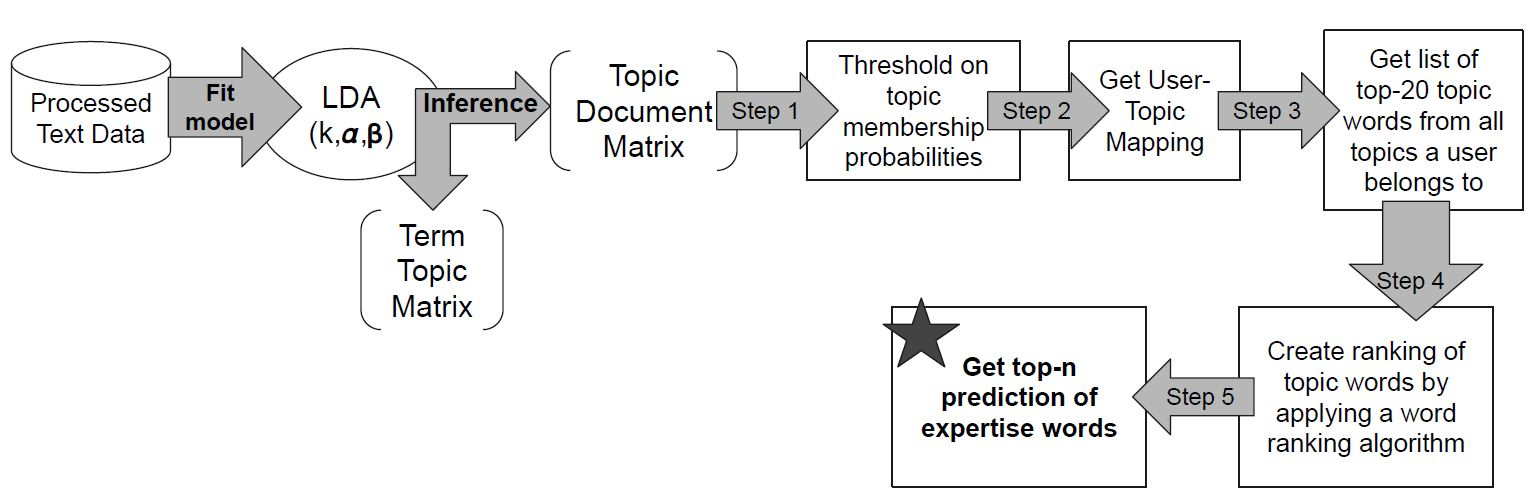
\includegraphics[width=\textwidth]{figures/technique1.JPG}\\
              \caption{Topic Distribution based Expertise Prediction}
              \label{fig:technique1}
            \end{figure}
            
        \subsubsection{Novel Technique 2: Expertise Prediction using LDA based User and Topic Embeddings}
        
            The second technique introduces the idea of generating user and topic embeddings in the same vector space, so their similarity could be computed. The creation of the user-topic mapping is accomplished by comparing cosine similarities between user and topic embeddings, thus associating a user with the most similar topics. 
            
            All unique words in a user profile are contributing to generate user embeddings using aggregated latent scores of each word present in the LDA model's term-topic matrix. The formal algorithm for \emph{LDA based User Embedding Generation} can be seen in Algorithm \ref{alg:LDA_userEmb}. 
            
            \begin{algorithm}
                \caption{LDA based User Embedding Generation}
                \label{alg:LDA_userEmb}
                \begin{algorithmic}[1]
                    \REQUIRE $M$: Term-Topic Matrix, $D$: User Profile Documents 
                    \STATE listOfEmbeddings = [ ]
                    \FORALL{users $user\_ID$ in the data set} 
                        \STATE Get user profile document $d$ for user $user\_ID$ from $D$
                        \STATE Get unique set words $WordSet$ in document $d$
                        \STATE listOfVectors = [ ]
                        \STATE
                        \FOR{each word $w$ in $WordSet$}
                            \STATE Get $1 \times k$ vector $v$ of latent scores for word $w$ from matrix $M$
                            \STATE Add vector $v$ to listOfVectors
                        \ENDFOR
                        \STATE Convert listOfVectors to matrix $LV$ with dimensions $n \times k$; $n=length(WordSet)$
                        \STATE Perform column-wise max-pooling or average-pooling to reduce matrix $LV$ to a user embedding vector $emb$, dimension $1 \times k$
                        \STATE Add user embedding vector $emb$ to listOfEmbeddings
                    \ENDFOR
                    \STATE Convert listOfEmbeddings to matrix $E$ with dimensions $u \times k$; where $u$ = number of users in the data set
                    \RETURN Matrix $E$
                \end{algorithmic}
            \end{algorithm}
        
            The \emph{LDA based User Embedding Generation} algorithm takes as input the collection of user profiles, and a term-topic matrix learned during inference of a fitted LDA topic model. In line 4 of Algorithm \ref{alg:LDA_userEmb} a set of words is created, which contains all the words appearing in a user's profile. In lines 7-10 this set of words is iterated over, and for each word a vector of latent scores is obtained from the input term-topic matrix. In line 12 a column-wise aggregation is performed by applying either max-pooling or average-pooling down-sampling technique. Applying a column-wise average or maximum function is a common word embedding aggregation technique \cite{de2016representation} used to create feature vectors from word embeddings. There are 2 variations of Algorithm \ref{alg:LDA_userEmb}. In order to explore which down-sampling technique works best experiments have been performed using both max and average-pooling, thus obtaining a convenient $1 \times k$ user embedding vector for each user.
                    
            Topic embeddings are generated using aggregated latent scores of top-20 topic words of each topic present in a fitted LDA model. The formal algorithm for \emph{LDA based Topic Embedding Generation} can be seen in Algorithm \ref{alg:LDA_topicEmb}. 
        
            \begin{algorithm}
                \caption{LDA based Topic Embedding Generation}
                \label{alg:LDA_topicEmb}
                \begin{algorithmic}[1]
                    \REQUIRE $LDA$: Topic Model, $M$: Term-Topic Matrix
                    \STATE listOfEmbeddings = [ ]
                    \FOR{each topic $T_i$ in $LDA$ fitted model} 
                        \STATE Get top-20 topic words $TW$ describing topic $T_i$
                        \STATE listOfVectors = [ ]
                        \STATE
                        \FOR{each word $w$ in $TW$}
                            \STATE Get $1 \times k$ vector $v$ of latent scores for word $w$ from matrix $M$
                            \STATE Add vector $v$ to listOfVectors
                        \ENDFOR
                        \STATE Convert listOfVectors to matrix $LV$ with dimensions $n \times k$; where $n=20$, $k=$ number of topics in $LDA$ model
                        \STATE Perform column-wise max-pooling or average-pooling to reduce matrix $LV$ to a topic embedding vector $emb$, dimension $1 \times k$
                        \STATE Add topic embedding vector $emb$ to listOfEmbeddings
                    \ENDFOR
                    \STATE Convert listOfEmbeddings to matrix $E$ with dimensions $k \times k$
                    \RETURN Matrix $E$
                \end{algorithmic}
            \end{algorithm}
            
            The \emph{LDA based Topic Embedding Generation} algorithm takes as input a fitted LDA model and the term-topic matrix learned during inference. In lines 2 and 3 of Algorithm \ref{alg:LDA_topicEmb} for each topic in the LDA model a set of top-20 topic words best representing that topic are obtained from the LDA model. In lines 6-19 this set of topic words is iterated over, and for each topic word a vector of latent scores is obtained from the input term-topic matrix. In line 11 a column-wise aggregation is performed by applying either max-pooling or average-pooling down-sampling technique. Same as for the \emph{LDA based User Embedding Generation}, there are 2 variations of Algorithm \ref{alg:LDA_topicEmb} too, by applying both max and average-pooling, and experimenting which down-sampling technique works best. After applying this process for each topic, a convenient $1 \times k$ topic embedding vector is obtained.
            
            The prediction of expertise is accomplished through a collection of topic words representing topics that a user most likely belongs to based on thresholds applied to cosine similarities calculated between a user embedding and each topic embedding. The formal algorithm for the overall \emph{Expertise Prediction using LDA based User and Topic Embeddings} can be seen in Algorithm \ref{alg:LDA_emb}.
        
            \begin{algorithm}
                \caption{Expertise Prediction using LDA based User and Topic Embeddings}
                \label{alg:LDA_emb}
                \begin{algorithmic}[1]
                    \REQUIRE $D$: User Profile Documents, $LDA$: Topic Model, $threshold$: Cosine Similarity Threshold
                    \STATE Get Term-Topic Matrix $M$ learned during inference of fitted $LDA$ topic model
                    \STATE User-Topic Mapping = \{ \}
                    \STATE Expertise-Predictions = \{ \}
                    \STATE Run LDA based User Embedding Generation to get $UserEmb$ matrix
                    \STATE Run LDA based Topic Embedding Generation to get $TopicEmb$ matrix
                    \STATE
                    \FOR{each user embedding $U$ in $UserEmb$}
                        \STATE listOfTopics = [ ]
                        \STATE user\_to\_topic\_sim = [ ]
                        \FOR{each topic embedding $T$ in $TopicEmb$}
                            \STATE Computer cosine similarity $SIM$ between user embedding $U$ and topic embedding $T$
                            \STATE Add $SIM$ to user\_to\_topic\_sim
                        \ENDFOR
                        \STATE
                        \STATE Get list of topics $LT$ associated with non-zero cosine similarities in user\_to\_topic\_sim
                        \FOR{topic $t$ in $LT$}
                            \IF{user\_to\_topic\_sim[ $t$ ] $\geq threshold$} 
                                \STATE Add topic $t$ to listOfTopics
                            \ENDIF
                        \ENDFOR
                        \STATE Get $User\_ID$ associated with user embedding $U$
                        \STATE User-Topic Mapping[ $User\_ID$ ] = listOfTopics
                        
                        \STATE
                        \STATE // Extract expertise for each user
                        \STATE listOfWords = [ ]
                        \FORALL{topic $t$ in User-Topic Mapping[ $user\_ID$ ]} 
                            \STATE $TW$ = Get top-20 topic words that describe topic $t$
                            \STATE Add topic words $TW$ to listOfWords
                        \ENDFOR
                        \STATE Apply a word ranking algorithm to listOfWords
                        \STATE Expertise-Predictions[ $user\_ID$ ] = sorted listOfWords
                    \ENDFOR
                    \RETURN Expertise-Predictions
                \end{algorithmic}
            \end{algorithm}
                
            The \emph{Expertise Prediction using LDA based User and Topic Embeddings} algorithm takes as input the collection of user profiles, an already fitted $LDA$ topic model, and a cosine similarity threshold, which is value strictly between 0 and 1. After getting the term-topic matrix from the $LDA$ model, Algorithm \ref{alg:LDA_userEmb} and \ref{alg:LDA_topicEmb} are executed to generate user and topic embeddings. Line 7 of Algorithm \ref{alg:LDA_emb} represents the iteration over each user embedding. In line 11 and 12 the cosine similarities between a user embedding and each topic embedding are calculated and stored. In line 15 the non-zero cosine similarities previously calculated are associated with similarities between a user and a topic. In lines 16-20 a topic becomes associated with a user if the cosine similarity between their respective embeddings is larger than or equal to the input cosine similarity threshold value. In lines 26-29 the top-20 topic words from each topic associated with a user are collected into a list of candidate expertise prediction words. Next, a ranking of the candidate expertise prediction words is created by applying the same word ranking metric used in Algorithm \ref{alg:Topic_Distr}, \emph{relevance}. Same as in the first novel technique, once the candidate expertise prediction words have been ranked, the top-$n$ ranked words are returned as the expertise words describing a user. A step-by-step visualization of the entire Algorithm \ref{alg:LDA_emb} can be seen in figure \ref{fig:technique2}.
             
            \begin{figure}[!ht]
              \centering
              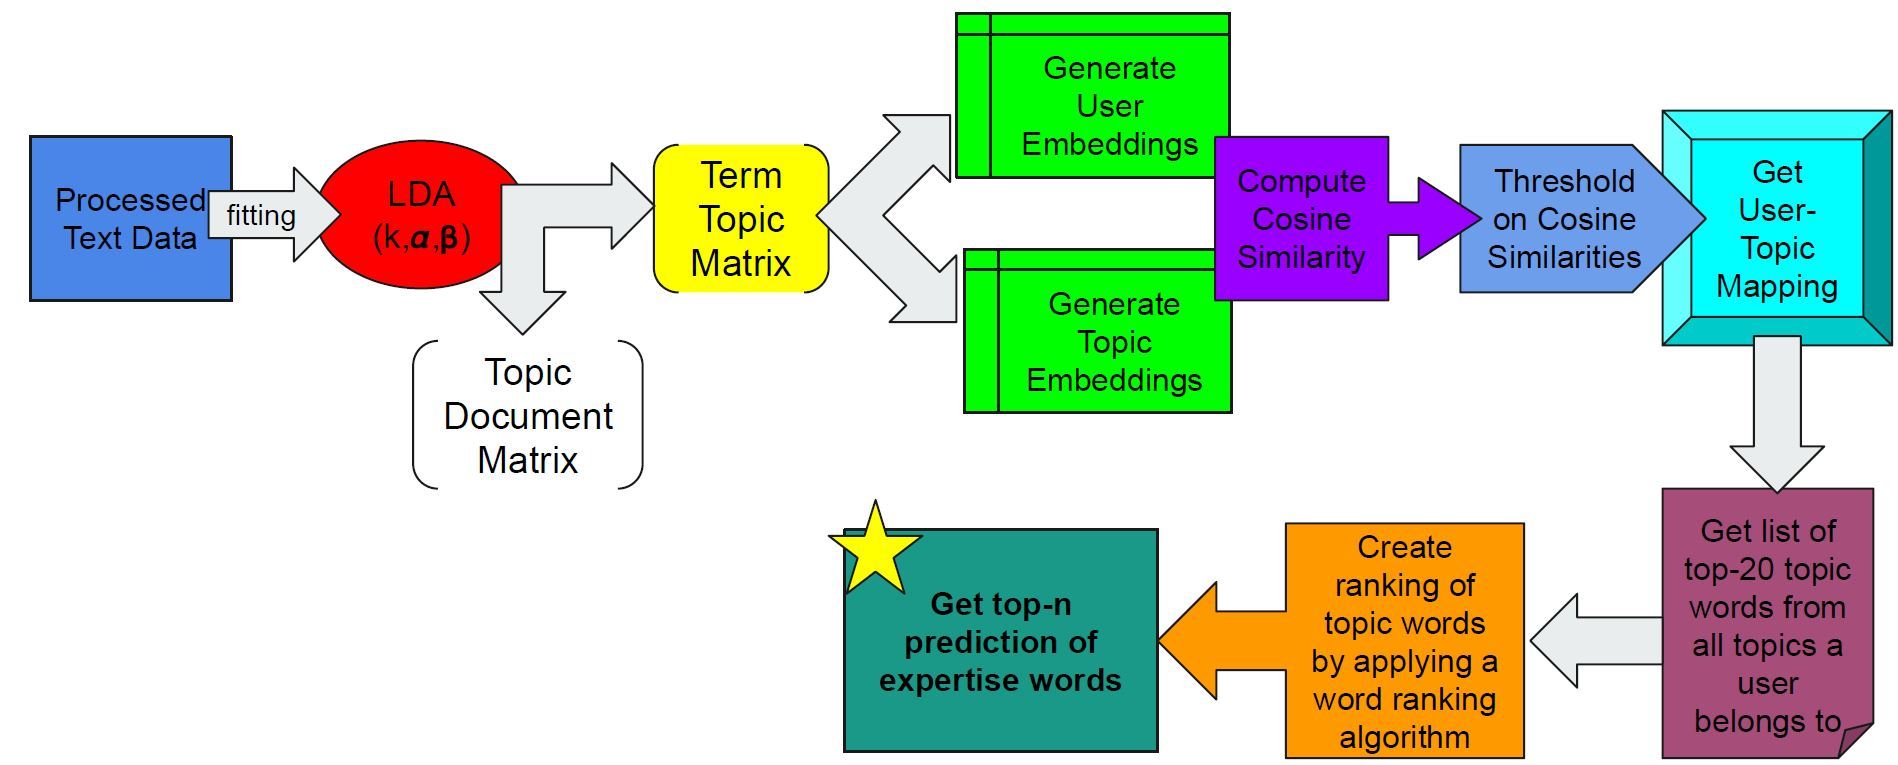
\includegraphics[width=\textwidth]{figures/technique2.JPG}\\
              \caption{Expertise Prediction using LDA based User and Topic Embeddings}
              \label{fig:technique2}
            \end{figure}
            
        \subsubsection{Novel Technique 3: Expertise Prediction using Pre-trained Word2Vec based User and Topic Embeddings}
        
            The third and last novel technique is a one step change on the second technique, \emph{Expertise Prediction using LDA based User and Topic Embeddings}. The only difference is that the LDA based latent score representation of words is replaced by continuous vector representation of words coming from pre-trained Word2Vec model. This model is publicly available, as it is Efstathiou et al. \cite{efstathiou2018word}'s work on \emph{Word Embeddings for the Software Engineering Domain}. The Word2Vec model \cite{mikolov2013efficient} was trained over 15GB of textual data from Stack Overflow posts, thus it captures software engineering specific contextual semantics. Making this change to technique 2 should be beneficial, as in theory the pre-trained Word2Vec model should provide better representation of words, from which better user and topic embeddings could be generated. The formal algorithms for the \emph{Pre-trained Word2Vec based User and Topic Embedding Generation} can been seen in Algorithms \ref{alg:Word2Vec_userEmb} and \ref{alg:Word2Vec_topicEmb}. Changes between the \emph{LDA based} and \emph{Pre-trained Word2Vec based} User and Topic Embedding Generation algorithms are highlighted with the color \textcolor{blue}{blue}. 
        
            \begin{algorithm}
            \caption{Pre-trained Word2Vec based User Embedding Generation}
            \label{alg:Word2Vec_userEmb}
            \begin{algorithmic}[1]
                \REQUIRE $D$: User Profile Documents,\textcolor{blue}{$word2vec$: Pre-trained Model}
                \STATE listOfEmbeddings = [ ]
                \FORALL{users $user\_ID$ in the data set} 
                    \STATE Get user profile document $d$ for user $user\_ID$ from $D$
                    \STATE Get unique set words $WordSet$ in document $d$
                    \STATE listOfVectors = [ ]
                    \STATE
                    \FOR{each word $w$ in $WordSet$}
                        \STATE \textbf{\textcolor{blue}{Look up vector representation $v$ of word $w$ in pre-trained $word2vec$ model}}
                        \STATE Add vector $v$ to listOfVectors
                    \ENDFOR
                    \STATE Convert listOfVectors to matrix $LV$ with dimensions $n \times d$; $n=length(WordSet)$,\textcolor{blue}{$d=$ dimensionality of $word2vec$ model}
                    \STATE Perform column-wise max-pooling or average-pooling to reduce matrix $LV$ to a user embedding vector $emb$, dimension $1 \times d$
                    \STATE Add user embedding vector $emb$ to listOfEmbeddings
                \ENDFOR
                \STATE Convert listOfEmbeddings to matrix $E$ with dimensions $u \times d$; where $u$ = number of users in the data set
                \RETURN Matrix $E$
            \end{algorithmic}
            \end{algorithm}
            
             The \emph{Pre-trained Word2Vec based User Embedding Generation} algorithm takes as input all user profile documents, and a pre-trained word2vec model. In line 8 of Algorithm \ref{alg:Word2Vec_userEmb} a user profile's each word's Word2Vec vector representation is queried. Contrary to common practise, out of vocabulary words are not assigned a vector of 0's, but rather skipped, as it would falsify the average-pooling down-sampling results, which are obtained in line 12. The algorithm produces $1 \times d$ dimensional user embedding vectors, where $d$ is 200, as Efstathiou et al. \cite{efstathiou2018word} trained their model with vector dimensions of 200 features. In the end, a matrix with dimensions $u \times d$ is returned, where $u$ is the number of users in the data set.
        
            \begin{algorithm}
            \caption{Pre-trained Word2Vec based Topic Embedding Generation}
            \label{alg:Word2Vec_topicEmb}
            \begin{algorithmic}[1]
                \REQUIRE $LDA$: Topic Model,\textcolor{blue}{$word2vec$: Pre-trained Model}
                \STATE listOfEmbeddings = [ ]
                \FOR{each topic $T_i$ in $LDA$ fitted model} 
                    \STATE Get top-20 topic words $TW$ describing topic $T_i$
                    \STATE listOfVectors = [ ]
                    \STATE
                    \FOR{each word $w$ in $TW$}
                        \STATE \textbf{\textcolor{blue}{Look up vector representation $v$ of word $w$ in pre-trained $word2vec$ model}}
                        \STATE Add vector $v$ to listOfVectors
                    \ENDFOR
                    \STATE Convert listOfVectors to matrix $LV$ with dimensions $n \times d$; where $n=20$,\textcolor{blue}{$d =$  dimensionality of $word2vec$ model}
                    \STATE Perform column-wise max-pooling or average-pooling to reduce matrix $LV$ to a topic embedding vector $emb$, dimension $1 \times d$
                    \STATE Add topic embedding vector $emb$ to listOfEmbeddings
                \ENDFOR
                \STATE Convert listOfEmbeddings to matrix $E$ with dimensions $k \times d$,  $k$ = number of topics in $LDA$ model
                \RETURN Matrix $E$
            \end{algorithmic}
            \end{algorithm}
            
            The \emph{Pre-trained Word2Vec based Topic Embedding Generation} algorithm takes as input an $LDA$ topic model, and a pre-trained word2vec model. In line 7 of Algorithm \ref{alg:Word2Vec_topicEmb} each topic word's Word2Vec vector representation is queried. The algorithm produces $1 \times d$ dimensional topic embedding vectors, where $d$ is 200. In the end, a matrix with dimensions $k \times d$ is returned, where $k$ is the number of topics in the input $LDA$ model.
            
            The prediction of expertise for the third technique is the same process as in Algorithm \ref{alg:LDA_emb}. The formal algorithm for the overall \emph{Expertise Prediction using Pre-trained Word2Vec based User and Topic Embeddings} can be seen in Algorithm \ref{alg:word2vec_emb}.
        
            \begin{algorithm}
            \caption{Expertise Prediction using Pre-trained Word2Vec based User and Topic Embeddings}
            \label{alg:word2vec_emb}
            \begin{algorithmic}[1]
               \REQUIRE $D$: User Profile Documents, $LDA$: Topic Model, $threshold$: Cosine Similarity Threshold,\textcolor{blue}{$word2vec$: Pre-trained Model}
                \STATE Get Term-Topic Matrix $M$ learned during inference of fitted $LDA$ topic model
                \STATE User-Topic Mapping = \{ \}
                \STATE Expertise-Predictions = \{ \}
                \STATE \textbf{\textcolor{blue}{Run Word2Vec based User Embedding Generation to get $UserEmb$ matrix}}
                \STATE \textbf{\textcolor{blue}{Run Word2Vec based Topic Embedding Generation to get $TopicEmb$ matrix}}
                \STATE
                \FOR{each user embedding $U$ in $UserEmb$}
                    \STATE listOfTopics = [ ]
                    \STATE user\_to\_topic\_sim = [ ]
                    \FOR{each topic embedding $T$ in $TopicEmb$}
                        \STATE Computer cosine similarity $SIM$ between user embedding $U$ and topic embedding $T$
                        \STATE Add $SIM$ to user\_to\_topic\_sim
                    \ENDFOR
                    \STATE
                    \STATE Get list of topics $LT$ associated with non-zero cosine similarities in user\_to\_topic\_sim
                    \FOR{topic $t$ in $LT$}
                        \IF{user\_to\_topic\_sim[ $t$ ] $\geq threshold$} 
                            \STATE Add topic $t$ to listOfTopics
                        \ENDIF
                    \ENDFOR
                    \STATE Get $User\_ID$ associated with user embedding $U$
                    \STATE User-Topic Mapping[ $User\_ID$ ] = listOfTopics
                    
                    \STATE
                    \STATE // Extract expertise for each user
                    \STATE listOfWords = [ ]
                    \FORALL{topic $t$ in User-Topic Mapping[ $user\_ID$ ]} 
                        \STATE $TW$ = Get top-20 topic words that describe topic $t$
                        \STATE Add topic words $TW$ to listOfWords
                    \ENDFOR
                    \STATE Apply a word ranking algorithm to listOfWords
                    \STATE Expertise-Predictions[ $user\_ID$ ] = sorted listOfWords
                \ENDFOR
                \RETURN Expertise-Predictions
            \end{algorithmic}
            \end{algorithm}
            
            The \emph{Expertise Prediction using Pre-trained Word2Vec based User and Topic Embeddings} algorithm takes as input the collection of user profiles, an already optimized, fitted $LDA$ topic model, and a cosine similarity threshold, $T$, which is a value strictly between 0 and 1. The only major change compared to the second technique is that in lines 4 and 5 Algorithms \ref{alg:Word2Vec_userEmb} and \ref{alg:Word2Vec_topicEmb} are executed to generate pre-trained Word2Vec based user and topic embeddings. The rest of the technique follows the same process as the second technique. A step-by-step visualization of the entire Algorithm \ref{alg:word2vec_emb} can be seen in figure \ref{fig:technique3}.
            
            \begin{figure}[!ht]
              \centering
              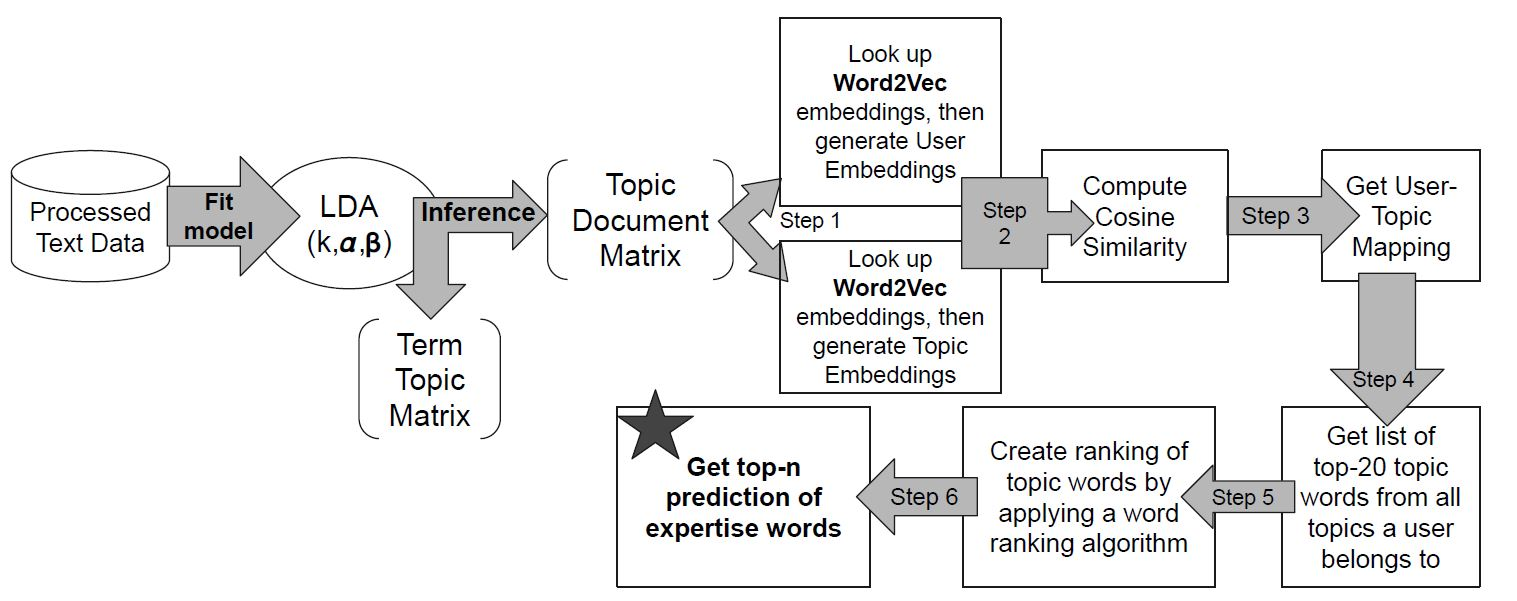
\includegraphics[width=\textwidth]{figures/technique3.JPG}\\
              \caption{Expertise Prediction using Word2Vec based User and Topic Embeddings}
              \label{fig:technique3}
            \end{figure}
        
        The above three techniques were carefully designed through multiple rounds of simulation and various changes to the implementation were performed. Algorithm \ref{alg:Topic_Distr}, \ref{alg:LDA_emb} and \ref{alg:word2vec_emb} presented above are the final versions that were proven to work the best. The most noteworthy change was considering topic probability or cosine similarity thresholding techniques instead of clustering users into similar groups. Algorithms such as \emph{k-means} and \emph{agglomerative} clustering were tested with to cluster user embeddings and topic embeddings in the same vector space. The theoretical idea was that user embeddings which get grouped into the same cluster as a topic embedding represent a user-topic association, thus a user would belong to the topic(s) that their user embedding got clustered into. This idea unfortunately did not work out, as the curse of dimensionality did not allow for meaningful clusters to be formed. Dimensionality reduction could have been applied through techniques such as PCA or t-SNE, but this was undesirable, since interpretation of cluster memberships was a priority, and interpreting principle components instead of any similarity scores was inconvenient. Furthermore, user and topic embeddings are already a form of down-sampling. Applying even further reduction of the data would create question about the validity of the techniques by too much loss of information due to dimensionality reduction. Instead, thresholding on topic probability and cosine similarity seemed the more ideal creation of user-topic association or mapping.
        
       \label{eval_expertise_prediction} To evaluate the performance of the above three techniques, four metrics have been considered: \emph{BLEU score, Jaccard similarity, Cosine similarity and F-score}. The formal definitions and more details about these metrics can be found in the Background chapter, section \ref{background:metrics}. When designing these techniques, the task seemed closer to text summarization, rather than a prediction task, as the human annotations summarize a developer's expertise area, thus BLEU score is a justified metrics. In this context the candidate summary is the model's set of prediction words, and the reference summary is the human annotation. When using \emph{BLEU scores}, the uni-gram matches only are taken into consideration. The similarity between the model's set of prediction words and the human annotation's set of words can be formulated into an word overlap formula, such as the one \emph{Jaccard similarity} has, thus this metric is also justified. In the evaluation of the above three techniques \emph{Cosine similarity} is used to compute a multi-word comparison between the model's prediction words and the human annotation's set of words, by using a pre-trained Word2Vec model\cite{efstathiou2018word} as a word vector representation look-up. Finally, \emph{F-score} is used to calculate the correct word matches between the model's set of prediction words and the human annotation's set of words.
       
       Subjectively, the most suited metric to the task of \emph{Expertise Prediction} should be \emph{Cosine similarity}, as it measures the semantic similarity between the two sets of words (annotation and model hypothesis), as opposed to counting how many words out the two sets of words are the same. \emph{Cosine similarity} as a metric would make the evaluation more robust, as opposed to making it a binary frequency count. All four metrics are reported to give a better sense of accuracy, but the \emph{Cosine similarity} score is the chosen evaluation metric.
        
        In order to compare each technique to a baseline, a random model was also created. This random model takes the text corpus' dictionary and calculates the frequency of each unique word in the corpus, then it normalizes them to create a frequency based discrete probability distribution. The random model samples $n$ words from the dictionary based on the probability distribution described above. The $n$ sampled words become the expertise prediction, thus defining a random baseline for the techniques. The goal is to outperform the random baseline as much as possible.
        
        Finally, as mentioned at the beginning of the subsection, comparing expertise trends on Stack Overflow and GitHub is still needed. After the best performing technique was found for both Stack Overflow and GitHub data sets, the best performing LDA model is extracted from the technique. The topics of these two LDA models fitted on Stack Overflow and GitHub are manually labelled based on the topic labeling methodology of Bangash et al. \cite{bangash2019developers} and Hindle et al. \cite{hindle2012relating}. The observations, trends and patterns noticed when comparing the topics of the two best performing models become the insight about expertise trends on Stack Overflow and GitHub.
     
        As mentioned at the beginning of section \ref{sec:algo_design}, the remainder of the subsections are focused on better understanding the modeling of expertise. The goal of these subsections was to perform analysis on LDA topics about expertise data and gain some insights into how cross-platform expertise is being developed on Stack Overflow and GitHub.
    
    \subsection{Cross-platform Expertise\label{RQ2_task}}
    
        This subsection is focused on comparing the expertise gained by the same users on Stack Overflow and GitHub. The goal is to explore to what extent do developers build similar expertise in Stack Overflow and GitHub? Will analysis show that there is knowledge transfer from one platform to another? To answer these questions, analysis is performed on four separate text corpora (GH-past, GH-recent, SO-past and SO-recent) which are explained in section \ref{past_recent_full_segm}. The set-up of the analysis is structured in a way to directly compare the expertise of the same user on GitHub and Stack Overflow, even in the same time. Two separate comparisons are considered: the text corpus of GH-past is compared with SO-past, and GH-recent is compared with SO-recent. The comparison takes shape by extracting key expertise terms of the same user from both Stack Overflow and GitHub user profiles, and comparing how much overlap there is in expertise terms of the same user on two different platforms. The formal algorithm used to extract expertise terms to be compared can be seen in Algorithm \ref{alg:RQ2}.
        
        \begin{algorithm}
            \caption{Extraction of Expertise Terms}
            \label{alg:RQ2}
            \begin{algorithmic}[1]
                \REQUIRE $Corpus\_1$: First Text Corpus, $Corpus\_2$: Second Text Corpus, $LDA\_Model$: Topic Model Fitted on the First Corpus
                \STATE Get common topic distribution $TD1$ for $Corpus\_1$ from the fitted $LDA\_Model$
                \STATE Get common topic distribution $TD2$ for $Corpus\_2$ by performing inference using the fitted topic model, $LDA\_Model$
                \STATE Expertise-Terms\_1 = \{ \}
                \STATE Expertise-Terms\_2 = \{ \}
                \STATE
                \STATE // For each user get expertise terms from $TD1$ and $TD2$ 
                \FORALL{users $user\_ID$ in the data set} 
                    \STATE listOf\_topicWords = [ ]
                    \FORALL{topics $t$ in $TD1$[ $user\_ID$ ] with probability $\geq 0.1$}
                        \STATE $TW$ = Get top-20 Topic Words representing topic $t$
                        \STATE Add Topic Words $TW$ to listOf\_topicWords 
                    \ENDFOR
                    \STATE Expertise-Terms\_1 [ $user\_ID$ ] = listOf\_topicWords
                    \STATE
                    
                    \STATE listOf\_topicWords = [ ]
                    \FORALL{topics $t$ in $TD2$[ $user\_ID$ ] with probability $\geq 0.1$}
                        \STATE $TW$ = Get top-20 Topic Words representing topic $t$
                        \STATE Add Topic Words $TW$ to listOf\_topicWords 
                    \ENDFOR
                    \STATE Expertise-Terms\_2 [ $user\_ID$ ] = listOf\_topicWords
                    \STATE
                \ENDFOR
                \RETURN Expertise-Terms\_1, Expertise-Terms\_2
            \end{algorithmic}
        \end{algorithm}
        
        The \emph{Extraction of Expertise Terms} algorithm takes in three parameters: the first and second text corpus, and the LDA model fitted on first text corpus. In line 1 of Algorithm \ref{alg:RQ2} the first topic document matrix ($TD1$) containing the topic distribution of each document in $Corpus\_1$ is obtained from the fitted $LDA\_Model$. In line 2 the second topic document matrix ($TD2$) is obtained by performing inference on $Corpus\_2$'s documents using the fitted $LDA\_Model$. This is a crucial step of the algorithm, as two topic distributions coming from two separate models can not be compared in the same analysis. Using bayesian inference on the second corpus allows both corpora to have a common topic distribution coming from a single fitted $LDA\_Model$. In line 7 an iteration of all users within the data set is performed. In lines 8-13 a list of all relevant expertise terms for $Corpus\_1$'s topic distribution is constructed. In line 9,  $TD1$[ $user\_ID$ ] represents the topic distribution of $user\_ID$'s user profile found in $Corpus\_1$. In the same line the iteration over all topics $t$ in $TD1$[ $user\_ID$ ] with probability greater than 0.1 represents the extraction of relevant topics found in $user\_ID$'s topic distribution. In this context relevant topics were defined as topics that describe the expertise of a user with at least a probability value of 0.1 (or 10 \%). In line 10-11 the top-20 topic words of $TD1$[ $user\_ID$ ]'s relevant topics are extracted and stored in a list of topic words, which become the expertise terms extracted from $Corpus\_1$'s topic distribution. In lines 15-20 the same process is applied to $Corpus\_2$'s documents. In line 16  $TD2$[ $user\_ID$ ] represents the topic distribution of $user\_ID$'s user profile found in $Corpus\_2$. In line 17-18 the top-20 topic words of $TD2$[ $user\_ID$ ]'s relevant topics are extracted and stored in a list of topic words, which become the expertise terms extracted from $Corpus\_2$'s topic distribution. At the end of the algorithm the expertise terms extracted from $Corpus\_1$ and $Corpus\_2$ are returned.
        
        The \emph{Extraction of Expertise Terms} algorithm is executed twice. In the first run the parameters were the GH-past and SO-past text corpora, and the GH-past LDA model. For the second run the GH-recent and SO-recent text corpora, and the GH-recent LDA model were passed as parameters. During both runs the LDA model is chosen based one whichever corpus has more data to train a larger LDA model. For both past and recent data segmentation the GitHub corpus is multiple times larger than the Stack Overflow one. Performing analysis on GH-past and SO-past text corpora, then on the GH-recent and SO-recent text corpora allows the direct expertise comparison of the same user on GitHub and Stack Overflow, in the same time. Once the expertise terms have been extracted, an iteration over all users is performed, and the \emph{Jaccard similarity} of the two sets of expertise terms is calculated. The \emph{Jaccard similarity} results are aggregated and interpreted using the help of histograms, density plots and bar plots in order to draw some insights about the extent that developers build similar cross-platform expertise.
    
    \subsection{Cross-platform Transferable Knowledge\label{RQ3_task}}
        This subsection is focused on discovering what knowledge is transferable from one platform to another? To answer this question the same analysis set-up as in section \ref{RQ2_task} is considered, as in the task of \emph{Cross-platform Expertise} the expertise of the same user is directly compared on GitHub and Stack Overflow. Performing the same experiment as in the previous task, but rather analyzing the \emph{Top-$n$} most frequent common expertise terms between the two platforms, for each user would shed some light on transferable knowledge.
        
        For the \emph{Cross-platform Transferable Knowledge} task the \emph{Extraction of Expertise Terms} algorithm is executed twice, with the \{GH-past, SO-past\}, and \{GH-recent, SO-recent\} text corpora pairs. The frequencies of common expertise terms in the text corpora pairs are calculated and the \emph{Top-$n$} common expertise terms, alongside with their frequency counts are returned. $n$ could take any value, but a larger value such as 50 or 100 would be considered appropriate. Any trends or patterns between the \emph{Top-$n$} common expertise terms are noted, then grouping of expertise terms into categories of transferable knowledge is performed. The patterns, trends, and groups of expertise terms become the insight gained into \emph{Cross-platform Transferable Knowledge}.
        
    \subsection{Expertise Evolution\label{RQ4_task}}
        
        This subsection is focused on comparing the evolution of expertise of same users on Stack Overflow and GitHub. The goal is to explore to what extent do developers' expertise change over time ? Furthermore, how is the evolution of expertise different on Stack Overflow and GitHub? To answer these questions, analysis is performed on four separate text corpora (GH-past, GH-recent, SO-past and SO-recent) which are explained in section \ref{past_recent_full_segm}. The set-up of the analysis is structured in a way to directly compare the expertise of the same user in the past and recent times, individually on GitHub, then on Stack Overflow. Two separate comparisons are considered: the text corpus of GH-past is compared with GH-recent, and SO-past is compared with SO-recent. The comparison is very similar to the one performed in section \ref{RQ2_task}, for \emph{Cross-platform Expertise}: expertise terms of the same user are extracted from both recent and past text corpora both Stack Overflow and GitHub data sets, Instead of comparing how much overlap there is in expertise terms of the same user (like section \ref{RQ2_task}), the opposite of overlap, difference or change in expertise terms of the same user is considered for the task of \emph{Expertise Evolution}. Since the task is concerned with expertise change over time, it seemed more appropriate to choose a metric that is related to dissimilarity of sets, which is  \emph{Jaccard distance}.
        
        Algorithm \ref{alg:RQ2}, the \emph{Extraction of Expertise Terms} was executed twice for the task of \emph{Expertise Evolution} too. In the first run the parameters were the GH-past and GH-recent text corpora, and the GH-past LDA model. For the second run the SO-past and SO-recent text corpora, and the SO-past LDA model were passed as parameters. During both runs the LDA model is chosen based one whichever corpus has more data to train a larger LDA model. For both GitHub and Stack Overflow data sets the past corpus segmentation is larger than the recent one. Performing analysis on GH-past and GH-recent text corpora, then on the SO-past and SO-recent text corpora allows the analysis of expertise evolution of the same user on GitHub, then on Stack Overflow independently. Once the expertise terms have been extracted, an iteration over all users is performed, and the \emph{Jaccard distance} of the two sets of expertise terms is calculated. The results are aggregated and interpreted using the help of histograms, density plots and bar plots in order to draw some insights about the extent that developers' expertise change over time.

\section{Software Tools Used} \label{sec:tools}
    Every algorithm described in section \ref{sec:algo_design} was implemented in Python 3.6 \footnote{\url{https://www.python.org/downloads/release/python-360/}}. The entirety of the data cleaning and processing stages, alongside the topic modeling was also done in Python. All implementations of common models and data science techniques come from open source Python libraries such as \emph{gensim}\footnote{for Topic Modeling - \url{https://radimrehurek.com/gensim/index.html}}, \emph{pyLDAvis}\footnote{Topic Modeling Visualization \url{https://pyldavis.readthedocs.io/en/latest/readme.html}}, \emph{numpy}\footnote{for Numpy Arrays - \url{https://numpy.org/}}, \emph{pandas}\footnote{for Data Structures - \url{https://pandas.pydata.org/}}, \emph{nltk}\footnote{for Textual Data - \url{https://www.nltk.org/}}, \emph{scikit-learn}\footnote{for Machine Learning - \url{https://scikit-learn.org/stable/index.html}}, \emph{scikit-optimize}\footnote{for Optimization - \url{https://scikit-optimize.github.io/}} and \emph{sqlalchemy}\footnote{for Database Connection - \url{https://www.sqlalchemy.org/}}. Occasionally Jupyter Notebooks\footnote{\url{https://jupyter.org}} were used on Google's Colaboratory \cite{bisong2019google} platform\footnote{Google Colab \url{https://colab.research.google.com}}. For data storage a MySQL database\footnote{\url{https://www.mysql.com/}} was chosen, and SQL was used to handle the data. All data plots were created using the R \cite{team2013r} statistical language's \emph{ggplot2} \cite{wickham2016ggplot2} library\footnote{\url{https://ggplot2.tidyverse.org/}}.


    
